%% Slides for ".NET Programming" by Chunyu Wang <chunyu@hit.edu.cn> %% -*- coding: utf-8 -*-

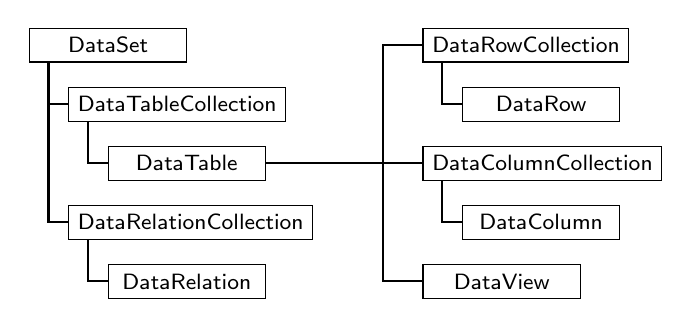
\begin{tikzpicture}
\tikzstyle{every node}=[anchor=west, draw, fill=white,
font=\sffamily\footnotesize, minimum width=2cm]
\foreach \x/\y/\t in 
  {0/4/DataSet, .5/3.25/DataTableCollection, 1/2.5/DataTable, .5/1.75/DataRelationCollection,
   1/1/DataRelation, 5/4/DataRowCollection, 5.5/3.25/DataRow, 5/2.5/DataColumnCollection,
   5.5/1.75/DataColumn, 5/1/DataView}
  \node at (\x,\y) (\t) {\t};
\draw[thick] (DataSet.south west) +(right:.25cm) |- (DataTableCollection);
\draw[thick] (DataTableCollection.south west) +(right:.25cm) |- (DataTable);
\draw[thick] (DataSet.south west) +(right:.25cm) |- (DataRelationCollection);
\draw[thick] (DataRelationCollection.south west) +(right:.25cm) |- (DataRelation);
\draw[thick] (DataTable.east) -- (4.5,2.5);
\draw[thick] (4.5,2.5) |- (DataRowCollection);
\draw[thick] (4.5,2.5) |- (DataColumnCollection);
\draw[thick] (4.5,2.5) |- (DataView);
\draw[thick] (DataRowCollection.south west) +(right:.25cm) |- (DataRow);
\draw[thick] (DataColumnCollection.south west) +(right:.25cm) |- (DataColumn);
\end{tikzpicture}
